\section{Notes d'histoire}

Louis Victor Leborgne, né en 1809 à Moret-sur-Loing commença à perdre la capacité de parler à l'age de 30 ans.
Il fut admis à l'hôpital de Bicêtre où il passerait 21 ans pendant lesquelles, 
il ne communiquait qu'en produisant le son ``tan'', typiquement répété deux fois, 
si bien qu'on lui a donné le surnom ``monsieur Tantan''~\cite{Mohammed_Narayan_Patra_Nanda_2018}.

Le 11 avril 1861, monsieur Leborgne fut examiné par Dr.~Pierre Paul Broca pour une gangrène dans son pied droit.
Dr.~Broca s'intéressa au trouble linguistique dont souffrait son patient~\cite{Lorch_2011}.
Il fit l'observation que les facultés intellectuelles et motrices de monsieur Leborgne étaient intactes,
il en conclut qu'elles ne peuvent être à l'origine de son handicape. 
Broca nomma ``aphémie'' ce type de situation~\cite{Broca}, il en écrivit :

\begin{quotation}
    ``Cette abolition de la parole, chez des individus qui ne sont ni paralysés ni idiots, constitue un symptôme assez singulier pour qu'il me paraisse utile de la désigner sous un nom spécial. Je lui donnerai donc le nom d'aphémie (\textgreek{a} privatif ; \textgreek{fhmi}, je parle, je prononce) ; car ce qui manque à ces malades, c'est seulement la faculté d'articuler les mots.''
    \begin{flushright}
        \rm --- \citeauthor{Broca}, 1861.
    \end{flushright}
\end{quotation}

Dr.~Broca prit ce constat comme confirmation de l'hypothèse de modularité du cerveau.
Il s'agit de l'idée que ce dernier fonctionne comme système à plusieurs composants plutôt qu'un monolithe
et que les fonctions cognitives sont spatialement localisées.

Quand monsieur Leborgne mourut le 17 avril, Dr.~Broca lui fit l'autopsie.
En ouvrant le crâne, il observa une lésion dans le cortex inférieur gauche du lobe frontale 
(Voire Figure~\ref{fig:leborgne-brain}).
Il en déduit (1) que cette lésion était à l'origine de l'aphémie de monsieur Leborgne et 
(2) que la partie affectée du cerveau est responsable d'articuler des expressions dans le langage
~\cite{Broca,Lorch_2011,Mohammed_Narayan_Patra_Nanda_2018}.

\begin{figure}[htb]
    \begin{center}
        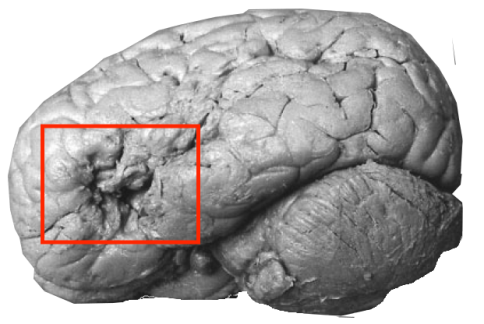
\includegraphics[width=10cm]{assets/images/leborgne-brain.png}
    \end{center}
    \caption{Cerveau de Victor Louis Leborgne avec la lésion encadrée}
    \label{fig:leborgne-brain}
\end{figure}